\documentclass[varwidth=true, border=2pt]{standalone}
\usepackage{tkz-euclide}

\begin{document}
\usetkzobj{all}
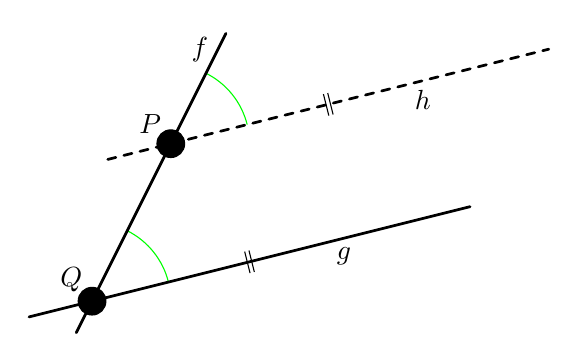
\begin{tikzpicture}
    \tkzSetUpPoint[shape=circle,size=10,color=black,fill=black]
    \tkzSetUpLine[line width=1]
    \tkzDefPoints{0/0/Q, 4/1/H1, 1/2/P}
    \tkzDefPoint(1.5,3){Phelper}
    \tkzMarkAngle[arc=l,size=1cm,color=green,fill=green!20](H1,Q,P)
    \tkzDrawLine(Q,H1)

    \tkzLabelPoint[above left](Q){$Q$}
    \tkzDefLine[parallel=through P](Q,H1) \tkzGetPoint{b}
    \tkzMarkAngle[arc=l,size=1cm,color=green,fill=green!20](b,P,Phelper)
    \tkzDrawLine[dashed](P,b)
    \tkzLabelLine[pos=0.8,below](P,b){$h$}
    \tkzLabelLine[pos=-0.6,left](P,Q){$f$}
    \tkzLabelLine[pos=0.8,below](Q,H1){$g$}
    \tkzLabelPoint[above left](P){$P$}
    \tkzDrawLine[add=0.2 and 0.7](Q,P)
    \tkzDrawPoints(P,Q)
    \tkzMarkSegments[mark=||](Q,H1 P,b)
\end{tikzpicture}
\end{document}
